
\documentclass[preprint,12pt]{elsarticle}

\usepackage[spanish]{babel}
\usepackage{amssymb}
\usepackage{graphicx}
\usepackage{lineno}
\usepackage[utf8]{inputenc}
\usepackage{url}
\usepackage{natbib}

\begin{document}
	
	\begin{frontmatter}

		\title{\huge  LABORATORIO N° 05: Elaboración de Reportes Operacionales	 }
		\author{	Tarqui Montalico,Risther(2017057469)}
		
		





\end{frontmatter}

%%INICIO Resumen
\section{Objetivo}
	
	Realizar con exito la elboracion de reportes operacionales, primero con un consultas en sql y luego con power BI 
%%FIN Resumen

\section{REQUERIMIENTOS }

	
		\begin{itemize}
			
			\\ \item Conocimientos
			Para el desarrollo de esta práctica se requerirá de los siguientes conocimientos básicos:
			\\ - Conocimientos básicos de administración de base de datos Microsoft SQL Server.
			\\ - Conocimientos básicos de SQL.
		\\ 	✓ Software
			\\ Asimismo se necesita los siguientes aplicativos:
			- Microsoft SQL Server 2017 o superior 
			
			
		\end{itemize}
	
	
\section

\section{DESARROLLO }


	\begin{itemize}
		
		\\ \item Parte 1: Debe crear la base de datos, tomando en cuenta las relaciones entre las
		tablas (llaves primarias y llaves foráneas). Así como se presenta en la siguiente
		figura:
		\\ 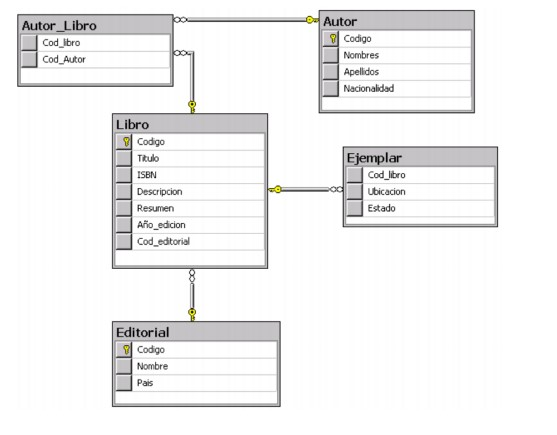
\includegraphics[width=7cm]{./IMAGENES/P1.1} 
		 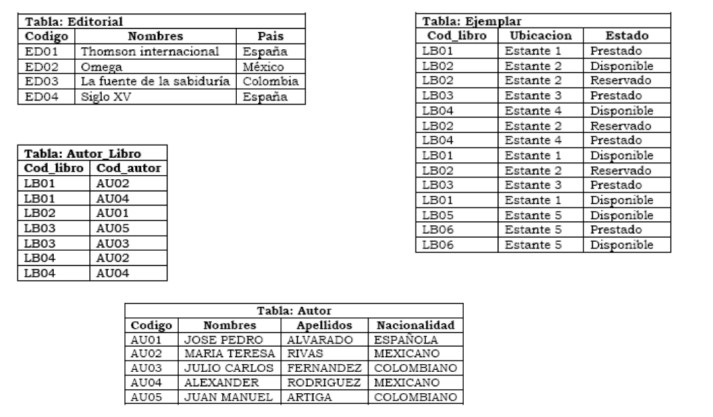
\includegraphics[width=7cm]{./IMAGENES/P1.2} \\
		\\ 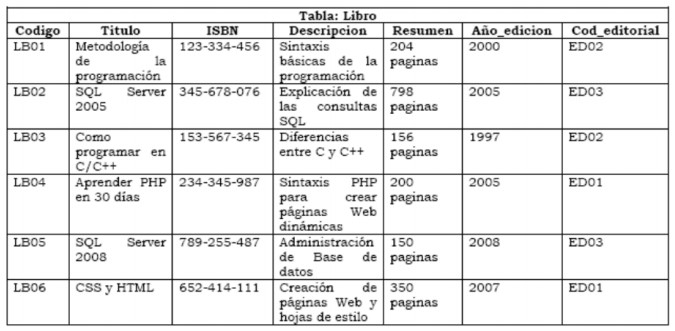
\includegraphics[width=7cm]{./IMAGENES/P1.3} \\
		
		\\ \item Parte 2: Crear las siguientes consultas SQL:
		Utilizando consultas a múltiples tablas resolver los siguientes problemas:
		\\ a. Se desea mostrar los datos de los autores junto con los títulos de libros que han escrito.
		Ordenarlos en forma descendente por el nombre del autor.
		\\
		\\ 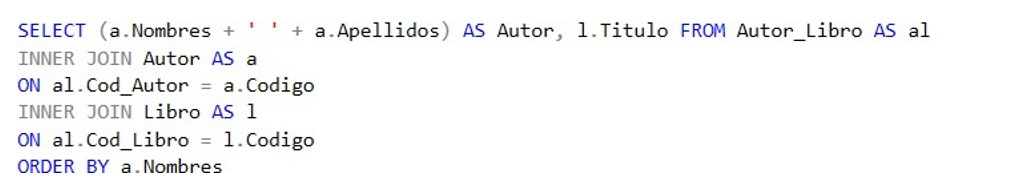
\includegraphics[width=7cm]{./IMAGENES/2.1} \\
		\\
		\\ 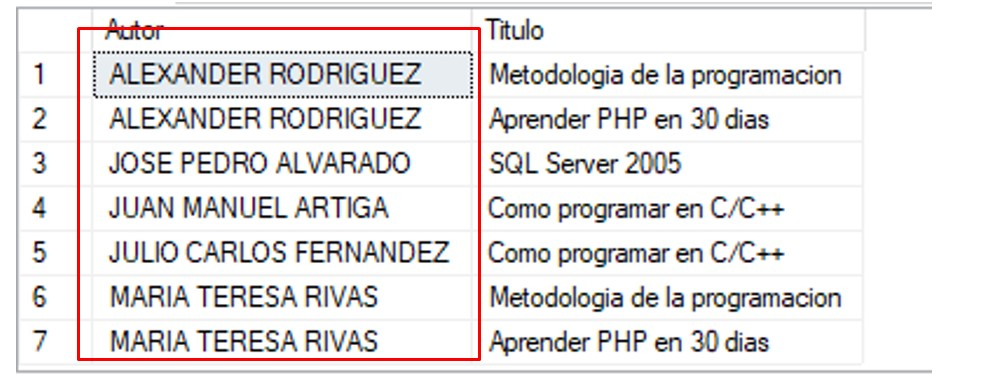
\includegraphics[width=7cm]{./IMAGENES/2.1.1} \\
		\\ b. Se desea conocer todos los autores que tienen libros que han sido publicados por la
		editorial “Omega”.
		\\
		\\ 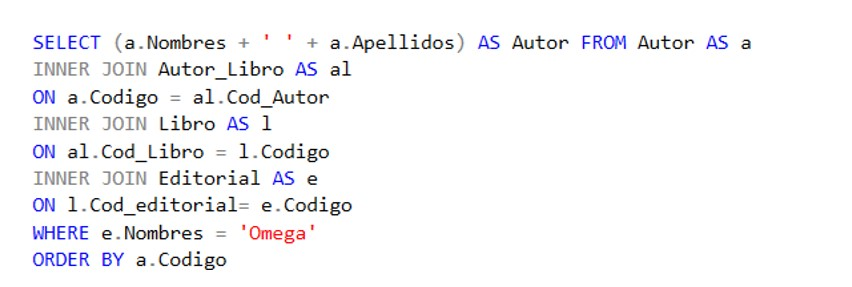
\includegraphics[width=7cm]{./IMAGENES/2.2} \\
		\\
		\\ 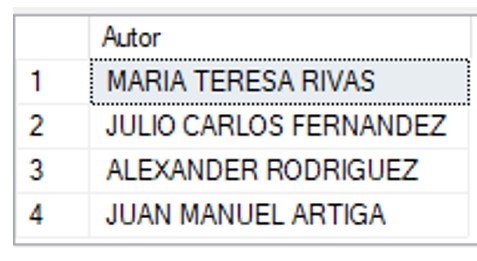
\includegraphics[width=7cm]{./IMAGENES/2.2.1} \\
		\\ c. Mostrar cuántos ejemplares hay por cada libro. Titulo, ejemplar
		\\
		\\ 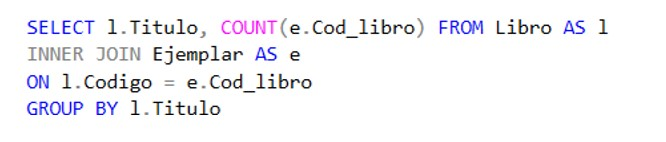
\includegraphics[width=7cm]{./IMAGENES/2.3} \\
		\\
		\\ 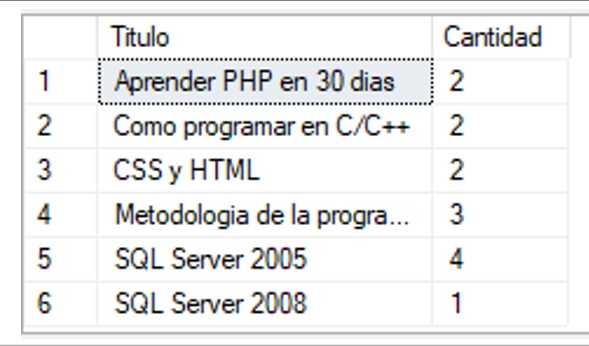
\includegraphics[width=7cm]{./IMAGENES/2.3.1} \\
		\\ d. Mostrar los títulos de los libros donde el estado sea “Prestado”.
		\\
		\\ 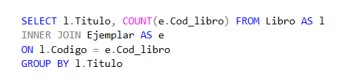
\includegraphics[width=7cm]{./IMAGENES/2.4} \\
		\\
		\\ 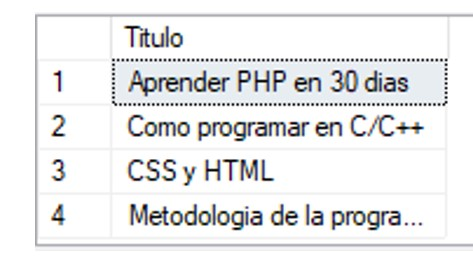
\includegraphics[width=7cm]{./IMAGENES/2.4.1} \\
		\\ e. Se desea mostrar los libros que se han editados entre el 2000 y 2007. Ordenarlos en
		forma ascendente.
		\\
		\\ 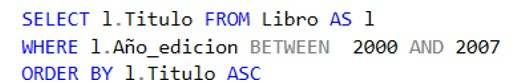
\includegraphics[width=7cm]{./IMAGENES/2.5} \\
		\\
		\\ 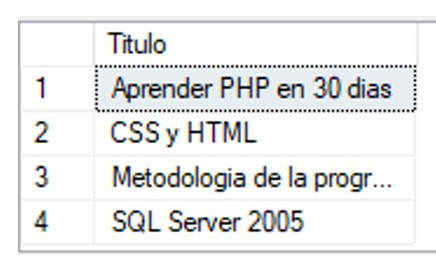
\includegraphics[width=7cm]{./IMAGENES/2.5.1} \\
		\\ f. Mostrar cuántos libros que se han prestado y agruparlos por el estante
		
		\\
		\\ 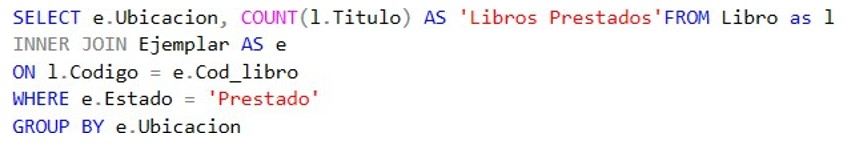
\includegraphics[width=7cm]{./IMAGENES/2.6} \\
		\\
		\\ 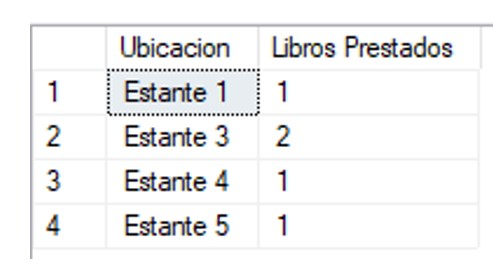
\includegraphics[width=7cm]{./IMAGENES/2.6.1} \\
		
		
		
		
		\\ \item Parte 3: Generar reportes operacionales de la parte II utilizando un visualizador Power BI, Tableau o
		Qlik Sense
		
	\\  	1.	Se desea mostrar los datos de los autores junto con los t´ıtulos de libros que han escrito.
		Ordenarlos en forma descendente por el nombre del autor
		\\ 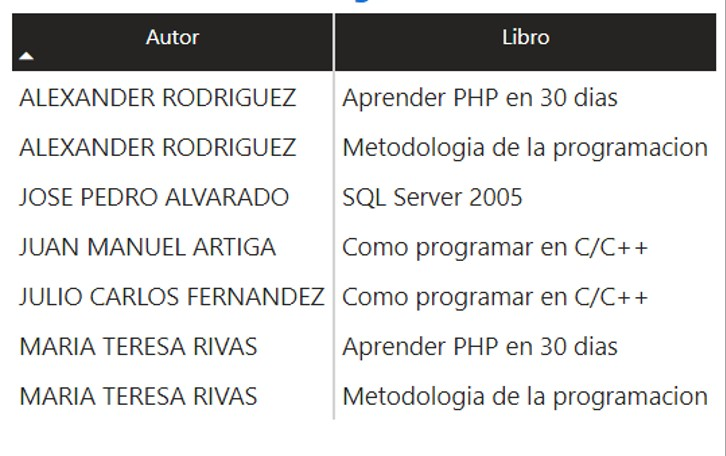
\includegraphics[width=7cm]{./IMAGENES/3.1} \\
		
	\\ \	2.	Se desea conocer todos los autores que tienen libros que han sido publicados por la editorial “Omega”.
		
			\\ 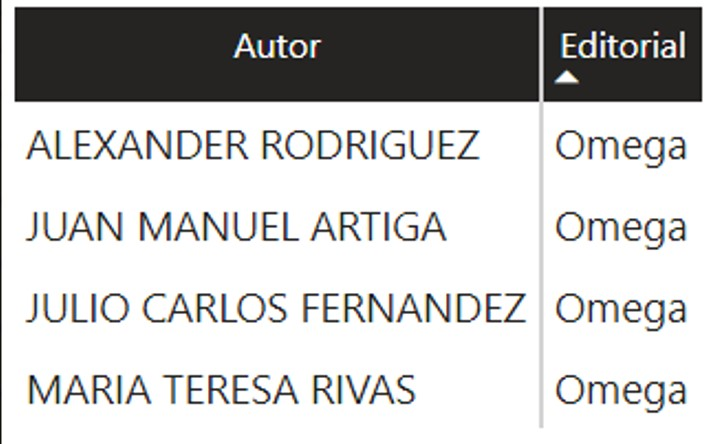
\includegraphics[width=7cm]{./IMAGENES/3.2} \\
	\\  	3.	Mostrar cu´antos ejemplares hay por cada libro.   Titulo, ejemplar.
			\\ 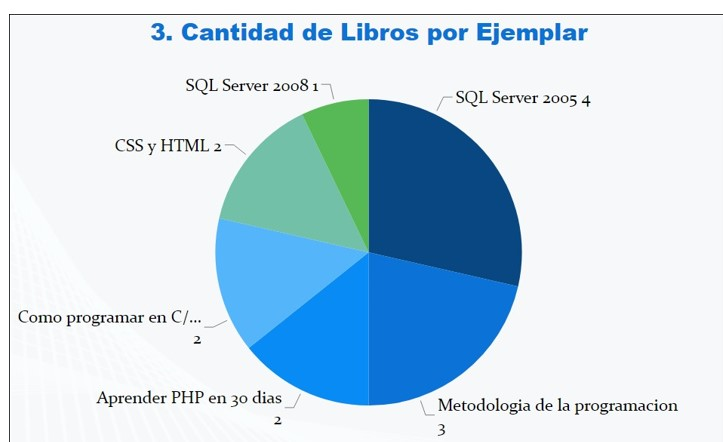
\includegraphics[width=7cm]{./IMAGENES/3.3} \\
		
	\\  	4.	Mostrar los   t´ıtulos de los libros donde el estado sea “Prestado”.
		\\ \includegraphics[width=7cm]{./IMAGENES/23.4} \\
	\\  	5.	Se desea mostrar los libros que se han editados entre el 2000 y 2007. Ordenarlos en forma ascendente.
		
			\\ 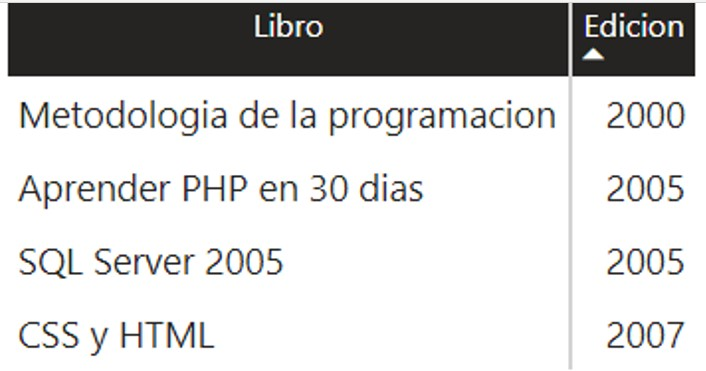
\includegraphics[width=7cm]{./IMAGENES/3.5} \\
	\\ 	6.	Mostrar cu´antos libros que se han prestado y agruparlos por el estante
		
			\\ 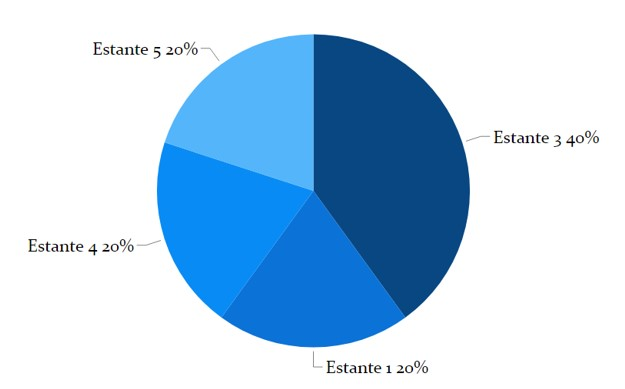
\includegraphics[width=7cm]{./IMAGENES/3.6} \\
	\\  	Finalmente nuestro dashboard se veria de la siguiente manera con todos los reportes solicitados.
		
			\\ 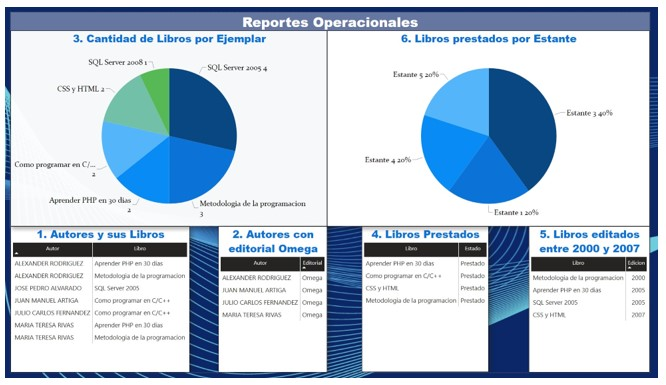
\includegraphics[width=7cm]{./IMAGENES/3.7} \\
	\end{itemize}


\section
%%INICIO Introducción

\section{Conclusiones}
		\begin{itemize}
		\item Se logro crear correctamente los reportes operacionales de la misma manera que se hizo con Queries en SQL Server que en un Visualizador de datos, en este caso Power BI, obteniendo los mismos resultados en ambos casos, pero es obvio que es mucho m´as entendible los resultados que nos ofrece el Power BI a diferencia del SQL Server que pocas podr´ıan comprender y tambi´en.
		\item Es mucho m´as sencillas elaborar los reportes en Power BI, ya que solo es cuesti´on de ir arrastrando los campos en los lugares que se crea necesaria de manera intuitiva a diferencia del SQL Server que se tiene que tener conocimiento b´asico para poder realizar las consultas.
		
		\end{itemize}
\section
%%----------------------------------------------------------------------------------------------------------------------------------------------------------



%CONCLUSIONES







	
	
%\citep{referenciarobles2}  


\end{document}

